\subsection{Graph Embedding}
\label{sec:design:subsec:embed}
% As we described in the previous section, the reinforcement learning agent must learn to choose two actions at each step in an epoch; the transformation and location from the set available dependent on the current computation graph. To learn the optimal action selection, we must create an embedding from the computation graph representation in the machine learning framework to our internal, manipulable graph representation inside our environment, our modified TASO backend.

When developing the project, a pivotal part of the project is the decision as to how we represent the GNN as there are a wide variety of forms which it can take. For example, a common implementation are message-passing networks (MPNNs) \cite{gilmer2017neural} which reduce data along edges and between nodes in the graph. Alternatively, we considered using graph convolutional networks (GCNs) \cite{kipf2016semi}, however, we found that using messages passing networks produced an adequate generalisable embedding that leverages the relational biases in the graph structure without added complexity of graph auto-encoders or graph convolution.

% [TODO] cite related work that used GNNs in Computer Systems

During training of the reinforcement learning agents, we convert the internal graph representation to a graph neural network. In order to train the model-free and model-based agents, a latent space embedding of the computation graph is required. Therefore, using the \texttt{graph\textunderscore nets} package developed by Battaglia et al. \cite{battaglia2018relational}, we implemented a graph neural network to learn a latent space embedding of the graph using message passing networks to gather the global learned features from the graph.

\begin{figure}[ht]
  \centering
  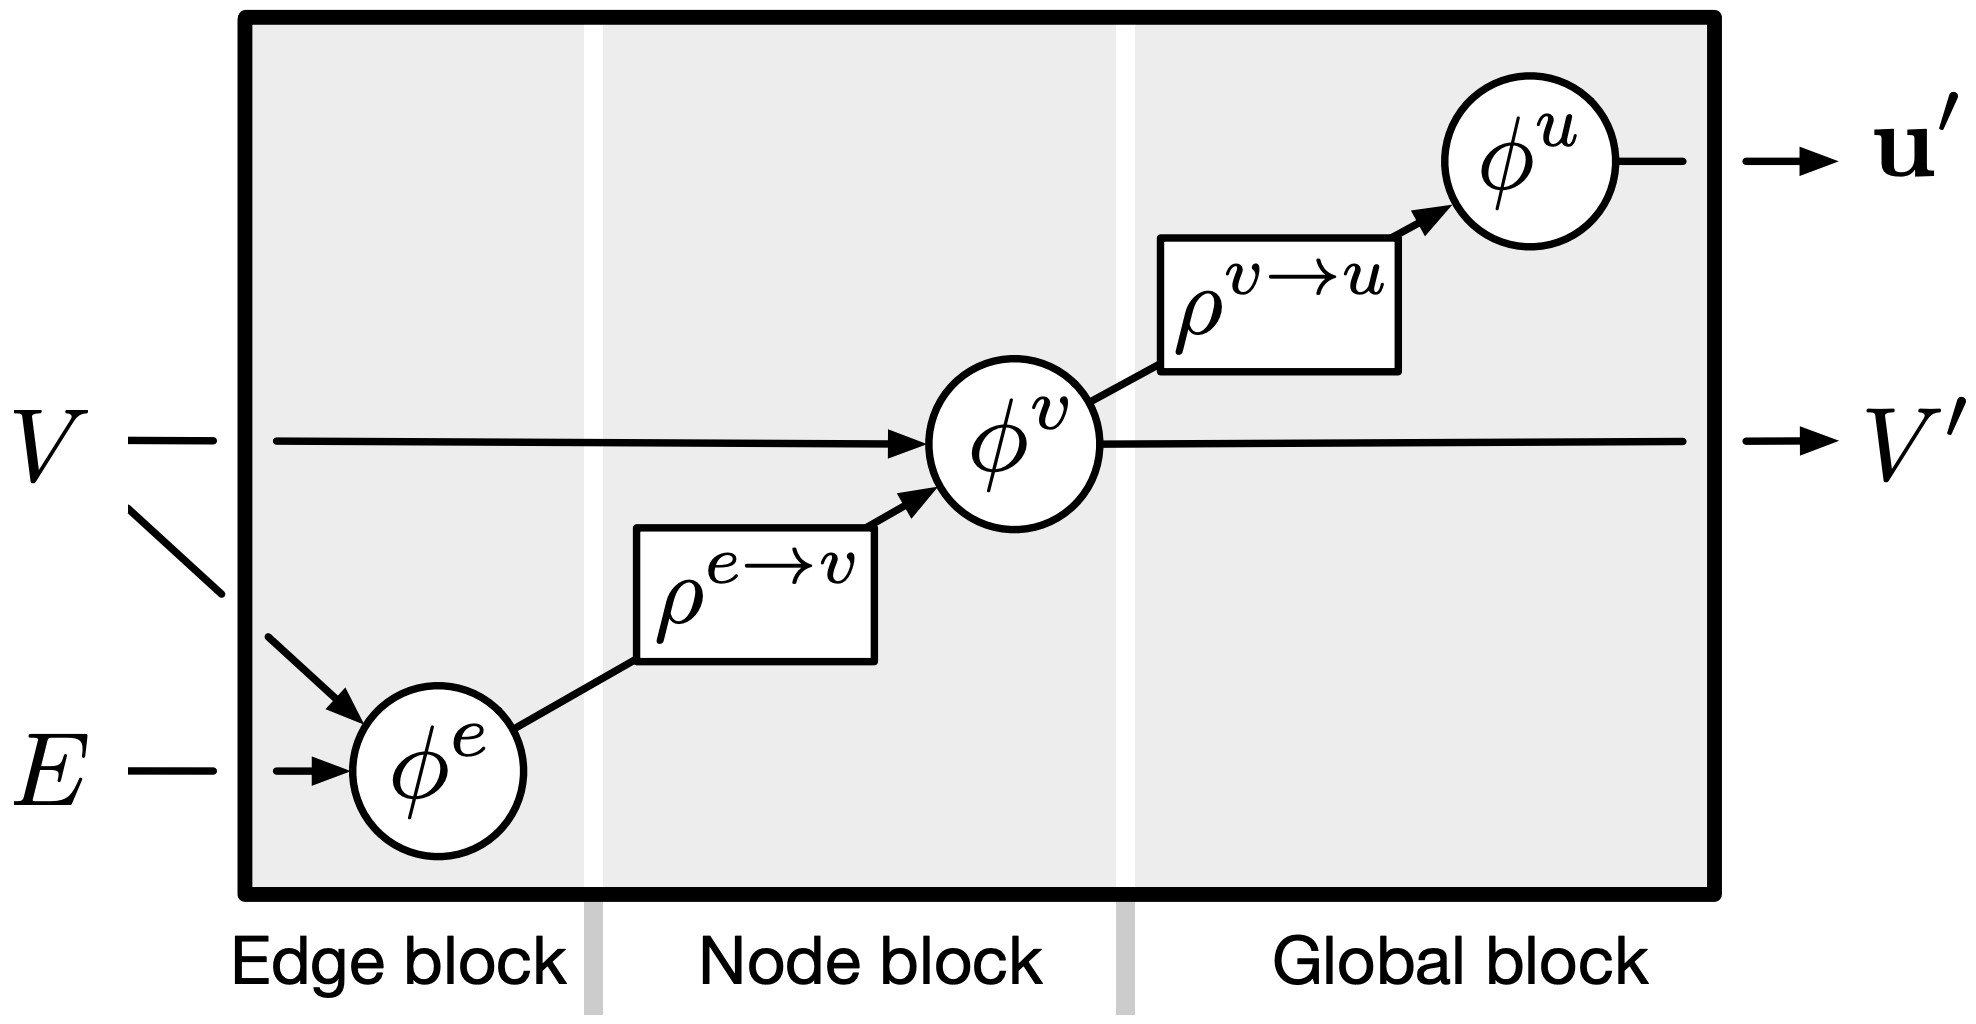
\includegraphics[width=0.75\columnwidth]{sections/4rlopt/images/mpnn.png}
  \caption[Message-passing neural network]{Message-passing Neural Network design using the three-step architecture described by \citet{battaglia2018relational}.}
  \label{fig:rlopt:mpgnn}
\end{figure}

As part of the design of the graph embedding network, we used a graph message passing neural network \cite{gilmer2017neural} that uses the input node, edge and global attributes to predict the node, edge and global attributes. In each of the five message passing rounds, we used an element-wise unsorted segment sum reduction function in the node block update of $\rho^{e\rightarrow v}$.

Furthermore, we acknowledge the work by Kai Fricke and Michael Schaarschmidt who developed the initial Python interface with TASO, the algorithm for converting the C++ TASO graph representation into a Cython object and performed experiments a model-free reinforcement learning agent \cite{xflowrl2019}. We used their work as a foundation upon which we continued development and research into model-free and model-based RL.
